\section{Maximum Three-Way Conference Rooms Tests}
\label{sec:conf-room}

Conference calls with fixed number of calls were developed primarily for executing three-way conferences.
Basically, there is a conference with y participants started. After that, there is another conference
with y participants started until the maximum number of conferences is reached:

\begin{figure} [!ht]
\centering
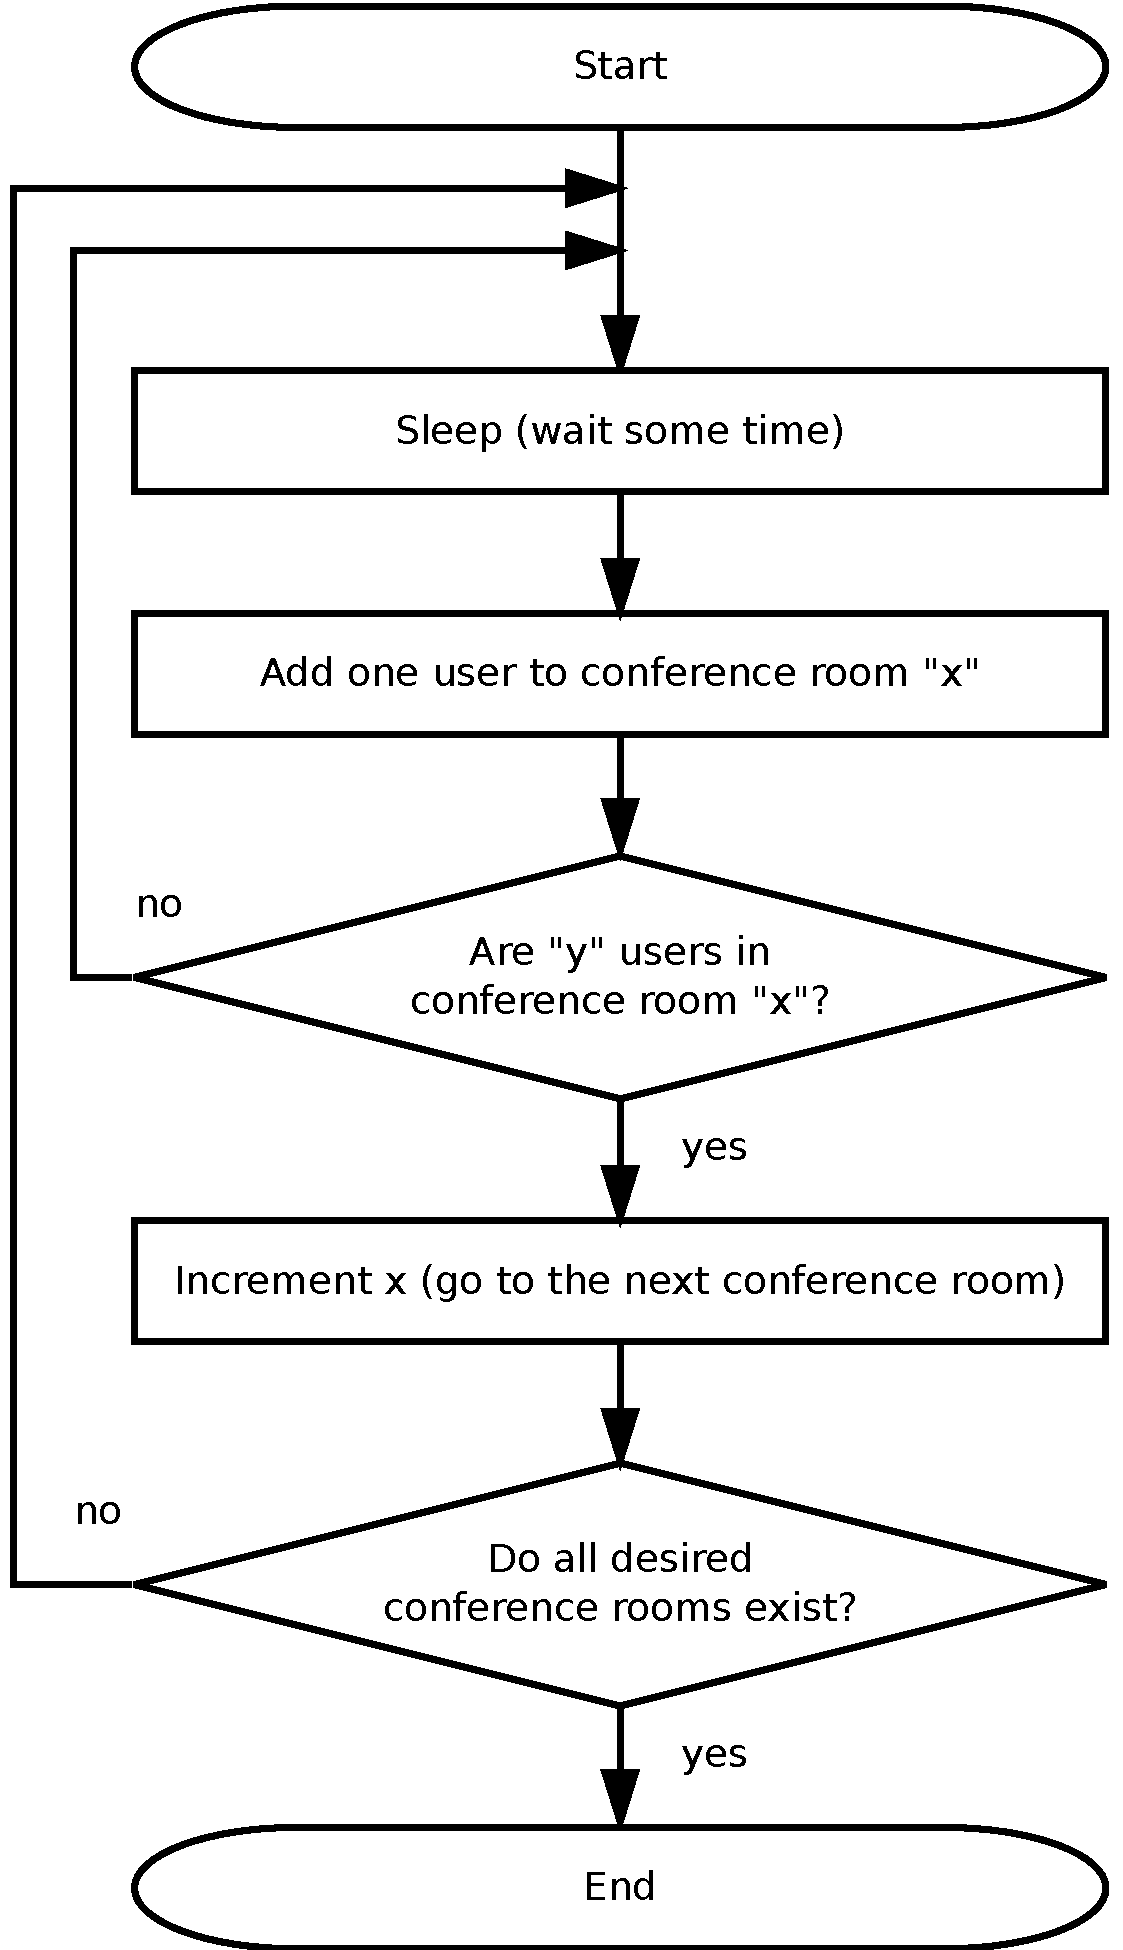
\includegraphics [width=8cm] {conf-call-1}
\caption{Process of conference call tests}
\end{figure}

For a conf call test with three participants and four conference rooms, the test would work like this: \newpage
\begin{figure} [!ht]
\centering
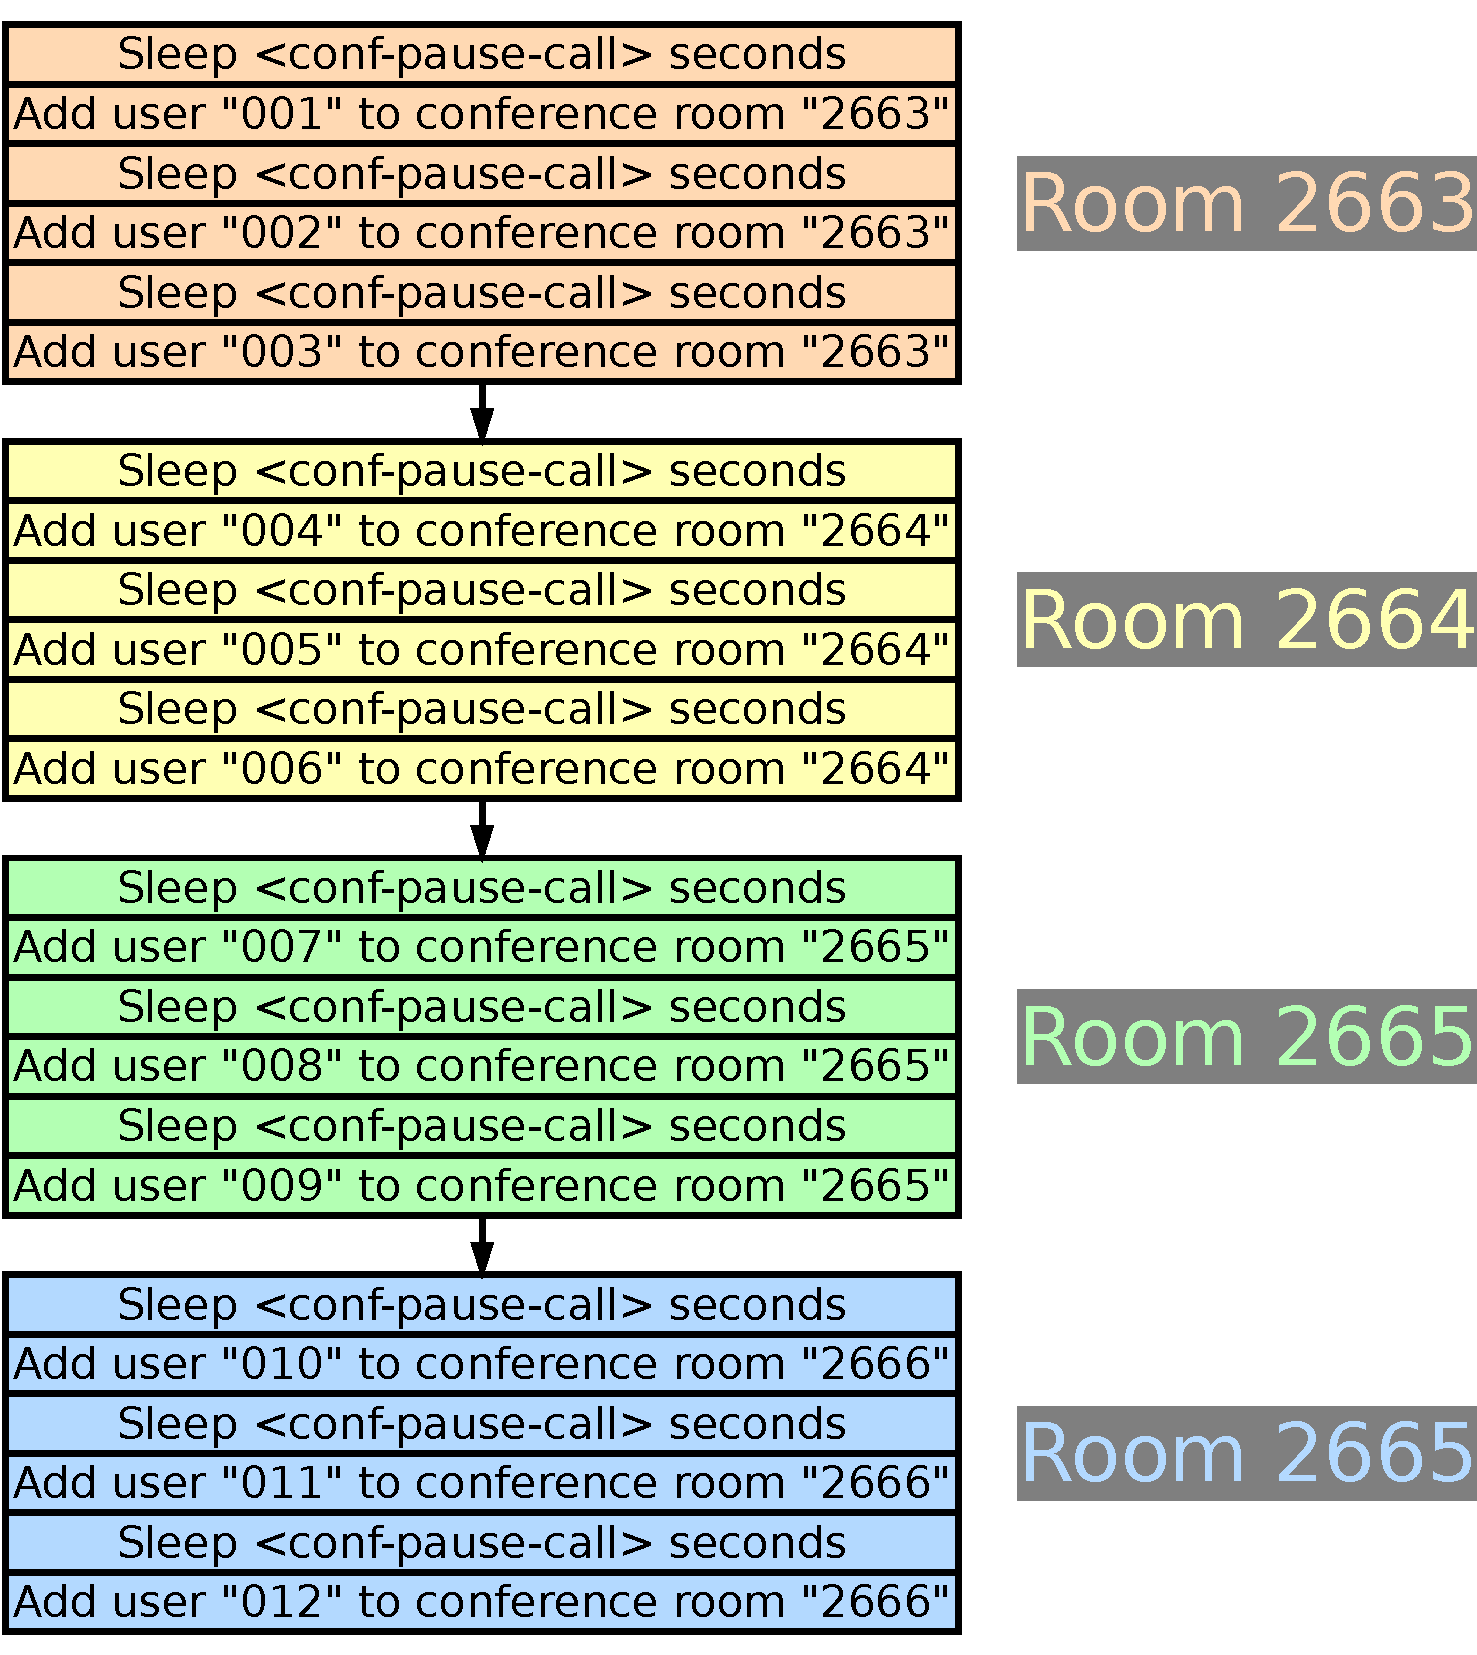
\includegraphics [width=8cm] {conf-call-2}
\caption{Conference call test example}
\end{figure}

This is implemented by using the sipp functionalities \texttt{call rates} (parameter -r)  and \texttt{rate period} (parameter -rp):
\begin{lstlisting}[breaklines=true,label=code:conf-call-invite,caption={sipp command for starting conf call tests} ]
"$sipp -aa -r 1 -i $local_ip
  -rp ". $conf_pause_call ."s 
  -inf '$users_conf_call_file'
  -m $current_users
  -p $sip_src_port
  -mp $rtp_src_port
  -sf '$inv_scen'
  $ask_ip 2>&1"
\end{lstlisting}

\texttt{-rp \$conf\_pause\_call s} is the rate period in seconds; it has to be \texttt{-rp 3s} or \texttt{-rp 10s} for example.
\texttt{-r 1 -rp \$conf\_pause\_call} means that 1 user is added every \texttt{conf-pause-call} seconds. 
In this case, the number of conference calls is tried to be kept constant. With this scenario, the following
situation is simulated (remember: each \texttt{conf-room} has \texttt{conf-calls} calls -- here, each of the 4 rooms has 3 calls):
\begin{figure} [!ht]
\centering
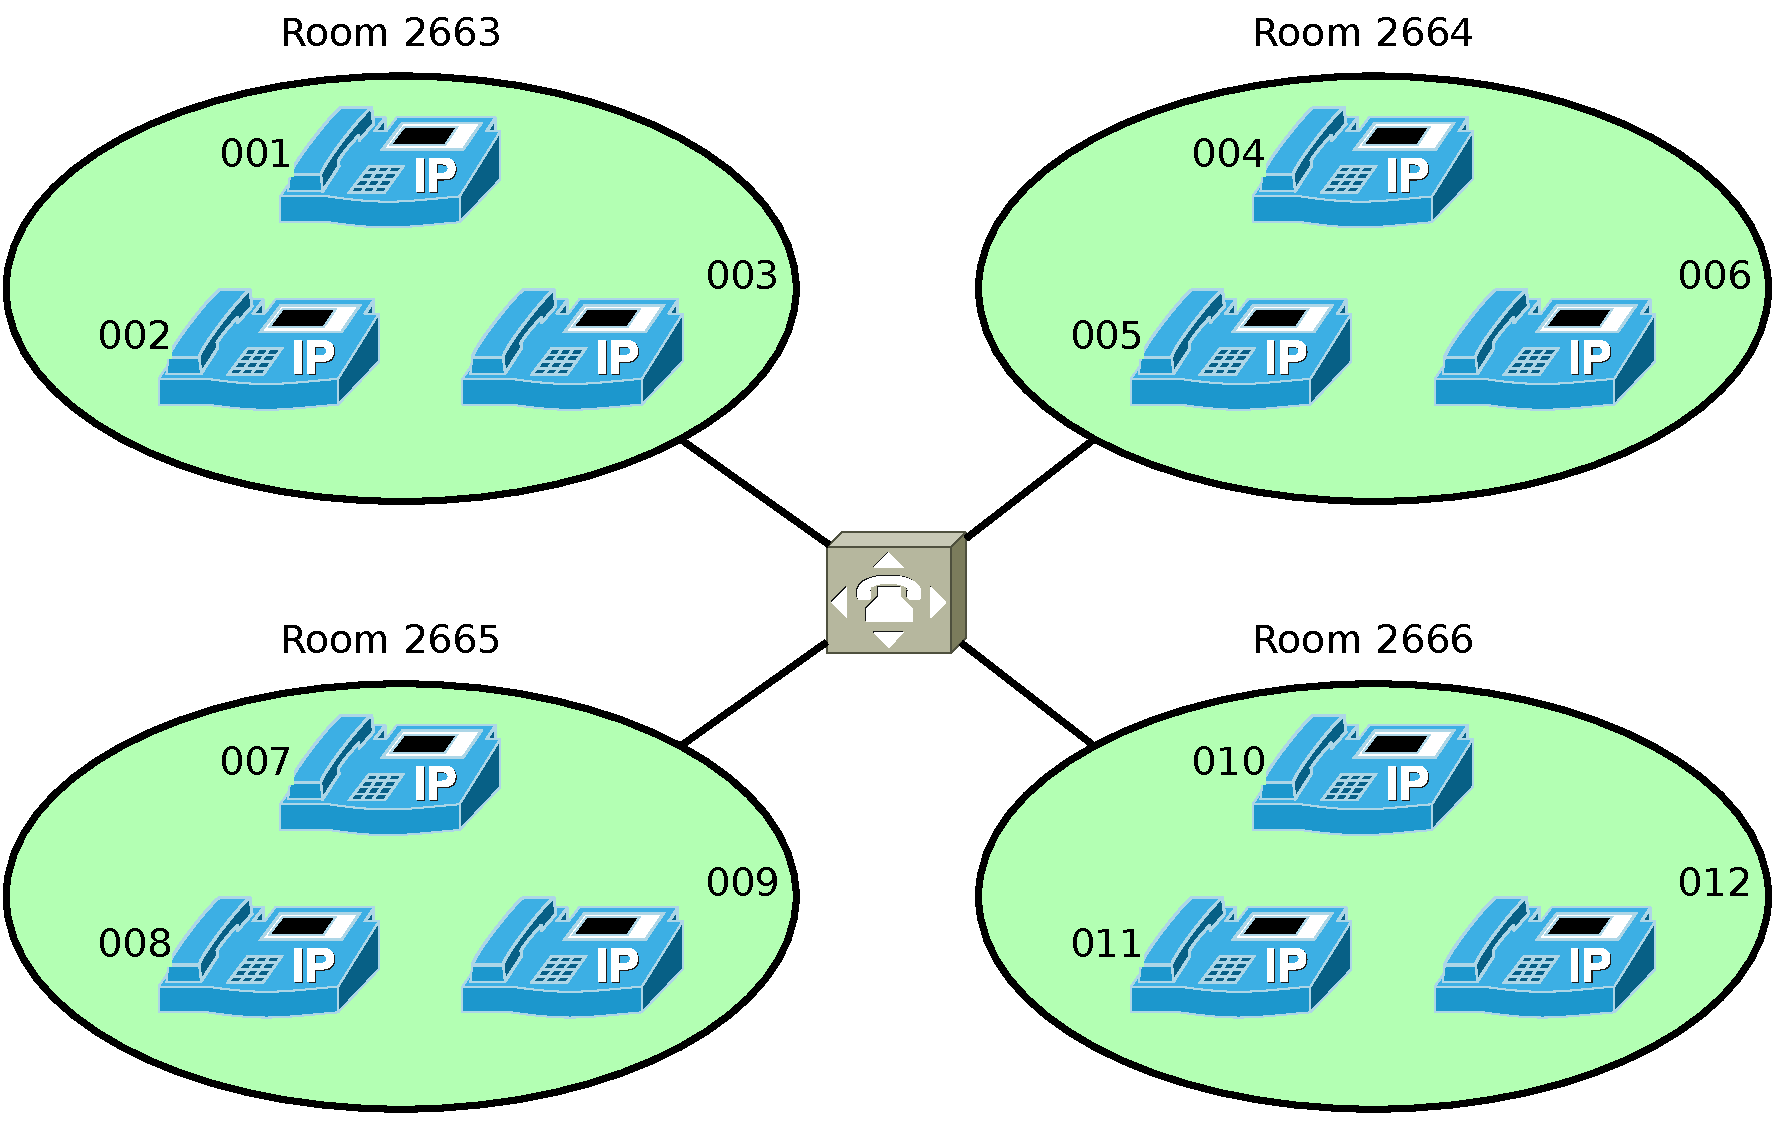
\includegraphics [width=10cm] {conf-call-3}
\caption {Conference call illustration with 3 calls, 4 rooms}
\label {fig:conf-call-illustration}
\end{figure}

